\chapter{Algoritmus A*}\label{A*}
Další možností, jak dohrát hru Snake, je stále hledat nejkratší možnou cestu od hlavy hada k jablku. Existuje mnoho algoritmů, kterými dokážeme najít nejkratší cestu z bodu A do bodu B, ale jedním z nejlepších je algoritmus A* (A - star). Tento algoritmus funguje na principu Dijkstrova algoritmu~\cite{Sharma2025Dijkstra}, ale ke zrychlení výpočtů využívá heuristiku. 

\section{Heuristika}
Proto abychom si lépe představili, co to heuristika je, uvedeme si příklad bludiště, kde na startu stojí myš a snaží se dostat na konec bludiště k sýru. Když se snaží myš dostat do cíle, tak může zvolit jakoukoli z možných cest. Tyto cesty mohou vést v lepším případě blíže k cíli, v horším ji zavedou naopak ještě dál od cíle, než byla na startu. Kdyby však cítila zápach sýru, věděla by vždy, jestli cítí zápach sýru méně, a tím pádem se vzdaluje, nebo jestli se zápach zesiluje a ona se k cíli naopak přibližuje (viz Obrázek~\ref{fig:MouseAndMaze}).

\begin{figure}[h]
    \centering
    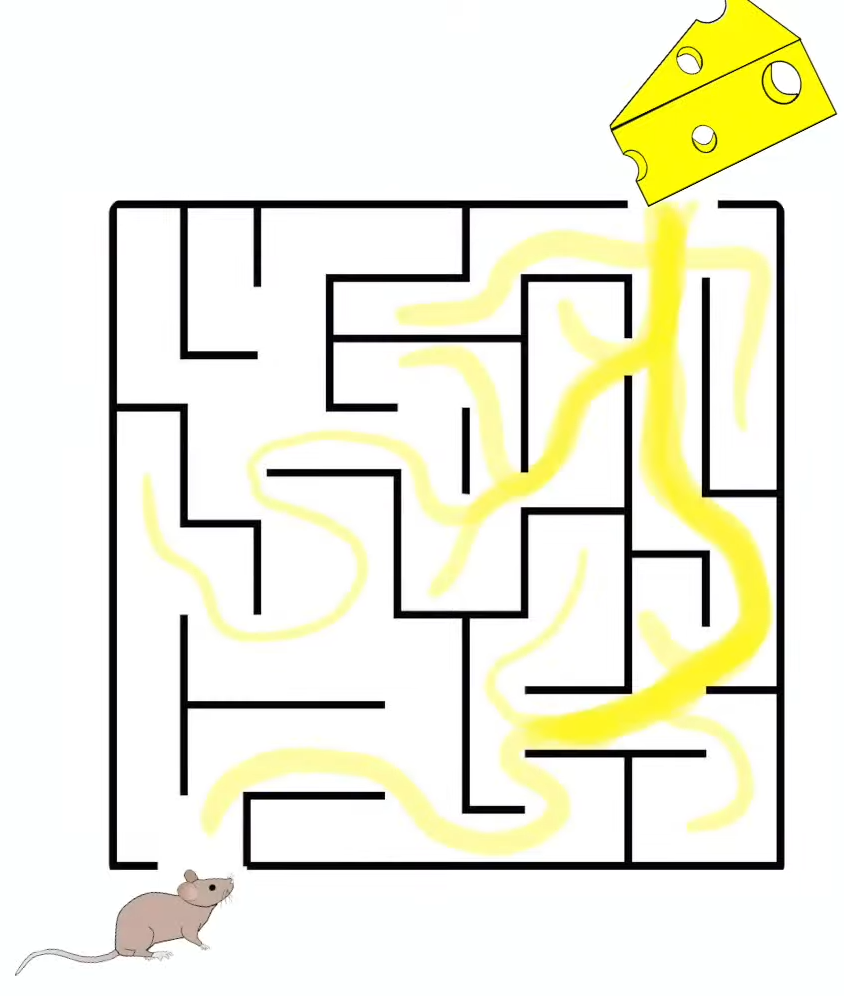
\includegraphics[width=0.5\linewidth]{Images/MouseAndMaze.png}
    \caption[Dostupné z: \url{https://www.youtube.com/watch?v=71CEj4gKDnE&ab_channel=AnishKrishnan}]{Myš a bludiště se sýrem (žluté čáry udávají intenzitu zápachu sýra)}
    \label{fig:MouseAndMaze}
\end{figure}

Díky tomu nemusí zkoušet cesty, které ji silně oddalují od cíle. Stále sice může vybrat cestu, která není správná, ale bude moci rychle rozpoznat, že tato cesta je špatná a vrátí se na tu správnou. V případě myši a sýru si můžeme heuristiku představit jako vůni, kterou myš cítí. Heuristika nám udává přibližný odhad toho, jak daleko jsme od cíle. 

V hracím poli pro hru Snake můžeme heuristiku reprezentovat jako Manhattanskou vzdále-\\nost, což je součet absolutních rozdílů souřadnic mezi dvěma body na mřížce. 

Matematicky ji lze vyjádřit jako:

\begin{center}
    \(d = |x_1 - x_2| + |y_1 - y_2|\),
\end{center}

kde (\(x_1, y_1\)) jsou souřadnice hlavy hada a (\(x_2, y_2\)) souřadnice jablka. Taková heuristika je pro náš problém vhodná, protože had se dokáže pohybovat pouze nahoru, dolů, doleva a doprava. 

\section{Popis algoritmu}

Jak již bylo zmíněno v úvodu kapitoly, algoritmus funguje na principu Dijkstrova algoritmu, má ale efektivnější výběr dalších vrcholů na zkoumání, ke kterému využívá heuristiku. V praxi se toho dosahuje prioritní frontou, ve které se vrcholy (\(V\)) řadí podle hodnoty \(f(V)\).

\(f(V)\) definujeme následně:

\begin{center}
    \(f(V) = g(V) + h(V)\),
\end{center}

kde \(g(V)\) je vzdálenost od počátečního vrcholu k mu vrcholu \(V\) a \(h(V)\) je heuristická vzdálenost od vrcholu \(V\) k cíli. 

Postup samotného algoritmu je následující (na jeho implementaci v pythonu lze nahlédnout v Ukázce kódu~\ref{lst:a_star}):

\begin{enumerate}
    \item Přidá počáteční vrchol do prioritní fronty s jeho \(f(V)\).
    \item Dokud fronta není prázdná, vrchol s nejnižší hodnotou \(f(V)\) bude z fronty vyřazen.
    \item Pokud je tento vrchol cíl, algoritmus se ukončí a vrátí zjištěnou cestu.
    \item V opačném případě se rozbalí uzel (najdou se všechny jeho sousedy) a vypočítají se \(g(V), h(V)\) a \(f(V)\) pro každého souseda. Každý soused se přidá do fronty, pokud tam ještě není, nebo pokud se k tomuto sousedovi nenajde lepší cesta.
    \item Cyklus se opakuje, dokud se nedojde k cíli nebo ve frontě už nezbyli žádné další uzly, což znamená, že neexistuje cesta od startu k vrcholu.
\end{enumerate}

\begin{figure}[H]
    \centering
    \begin{lstlisting}[language=python, style=python, caption={Implementace \(A^*\) v pythonu}, label={lst:a_star}, mathescape=true]
    def a_star(graph, start, goal):
        open_set = []
        # Push the start node with priority 0
        heapq.heappush(open_set, (0, start))
        came_from = {}
        # Cost from start to each node
        g_score = {node: float('inf') for node in graph}
        # Cost from start to start is 0
        g_score[start] = 0
        # Estimated total cost
        f_score = {node: float('inf') for node in graph}
        # Initial heuristic estimation
        f_score[start] = heuristic(start, goal)
    
        while open_set:
            # Get the node with the lowest f_score
            _, current = heapq.heappop(open_set)
            if current == goal:
                return reconstruct_path(came_from, current)
    
            for neighbor, cost in graph[current].items():
                tentative_g_score = g_score[current] + cost
                # If a better path is found
                if tentative_g_score < g_score[neighbor]:
                    came_from[neighbor] = current
                    g_score[neighbor] = tentative_g_score
                    f_score[neighbor] = g_score[neighbor] + heuristic(neighbor, goal)
                    heapq.heappush(open_set, (f_score[neighbor], neighbor))
        return None
    \end{lstlisting}
\end{figure}

\section{Nesprávnost řešení hry}

Použití algoritmu pro hledání nejkratší cesty od hlavy hada k jablku je sice z časového hlediska rozhodně rychlé, ale nikdy nedokáže zaplnit celé hrací pole, neboli úspěšně dohrát hru. Když se had bude postupně zvětšovat, bude na hracím poli méně volných políček a některá můžou být tělem hada kompletně odříznutá, kvůli čemuž had nabourá do sebe a zemře, aniž by zaplnil celé hrací pole. 

Pro objasnění si představme následující situaci. Had už je docela veliký a míří sníst další jablko. Cesta, kterou zvolil, oddělila část volných políček od ostatních. Nyní, když sní jablko a další se vygeneruje právě v tom odděleném prostoru, který v předchozích krocích vytvořil, neuvidí ho, neboli neexistuje žádná cesta od hlavy hada k jablku (viz Obrázek~\ref{fig:NoPathExistsHad}). Další případ, na kterém tento způsob kolabuje, je, když si had během pohybu k jablku odstřihne únikovou cestu, neboli cestu, po které by se mohl pohybovat zpátky poté, co jablko sní(viz Obrázek~\ref{fig:OdstrihnutiCestyHad}).

\begin{figure}[h]
    \centering
    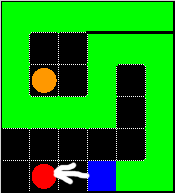
\includegraphics[width=0.4\linewidth]{Images/NoPathExistsHad.png}
    \caption{Had, který nemůže najít cestu k dalšímu vygenerovanému jablku, zelené čtverečky - tělo hada, modrý čtvereček - hlava hada, červené kolečko - jablko, které vidí aktuálně, oranžové kolečko - jablko, které uvidí poté co sebere červené jablko, bílá šipka - cesta, kterou had projde při hledání obou jablek}
    \label{fig:NoPathExistsHad}
\end{figure}

\begin{figure}[h]
    \centering
    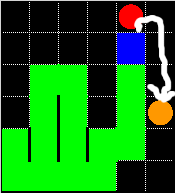
\includegraphics[width=0.4\linewidth]{Images/OdstrihnutiCestyHad.png}
    \caption{Had, který si zablokoval únikovou cestu, zelené čtverečky - tělo hada, modrý čtvereček - hlava hada, červené kolečko - jablko, které vidí aktuálně, oranžové kolečko - jablko, které uvidí poté co sebere červené jablko, bílá šipka - cesta, kterou had projde při hledání obou jablek}
    \label{fig:OdstrihnutiCestyHad}
\end{figure}